\documentclass[a4paper]{article}


\usepackage{alphabeta} 
\usepackage{enumitem} 
\usepackage{mathtools}
\usepackage{amsmath, amssymb} 
\usepackage{amsthm}
\usepackage{cancel} 
\usepackage[margin=0.70in]{geometry} 
\geometry{left=3cm,right=3cm,top=2.4cm,bottom=2.4cm}	%the page geometry as defined, A4=210x297mm
\usepackage{graphicx}
\usepackage{wrapfig}
\usepackage{caption}
\usepackage{textcomp}
\usepackage{tabto}
\usepackage{layout}
\usepackage{bm}
\usepackage{minipage-marginpar}
\usepackage[dvipsnames]{xcolor}
\usepackage{hyperref}
\usepackage{dutchcal}
\usepackage{derivative}
\usepackage{esint}
%\usepackage{biblatex}
\usepackage{subcaption}
\usepackage{booktabs}\usepackage{derivative}
\usepackage[flushleft]{threeparttable}
\usepackage[capbesideposition=outside,capbesidesep=quad]{floatrow}
\usepackage{derivative}
\usepackage[thinc]{esdiff}
\usepackage{lipsum}
\usepackage{arydshln}
%%RENEW

\newtheorem{problem}{Άσκηση}
\newtheorem*{solution*}{Λύση}
\newtheorem{definition}{Ορισμός}[subsection]
\newtheorem{properties}{Ιδιότητες}[subsection]
\newtheorem{theorem}{Θεώρημα}[subsection]
\newtheorem{protash}{Πρόταση}[subsection]
\newtheorem{porisma}{Πόρισμα}[subsection]
\newtheorem{lemma}{Λήμμα}[subsection]
\newtheorem*{prooof}{Απόδειξη}
\newtheorem*{notes}{Παρατηρήσεις}
\newtheorem*{note}{Παρατήρηση}
\newtheorem*{app}{Εφαρμογή} 
\newtheorem*{example}{Παράδειγμα}
\newtheorem*{examples}{Παραδείγματα}


\newcommand\numberthis{\addtocounter{equation}{1}\tag{\theequation}}
%\renewcommand{\labelenumi}{\roman{enumi}}
\newcommand{\approxtext}[1]{\ensuremath{\stackrel{\text{#1}}{\approx}}}
\renewcommand{\figurename}{Εικόνα.}
\renewcommand{\tablename}{Πίνακας.}
%\renewcommand\refname{New References Header}
\renewcommand*\contentsname{Περιεχόμενα}
%\DeclareDerivative{\odv}{\mathrm{d}}


\begin{document}
\begin{titlepage}			%makes a title page. Remember to change the author, CID, username and group number to what is appropriate for you!
	\centering
	{\scshape\LARGE Εθνικό Μετσόβιο Πολυτεχνείο\par}
	{\scshape \LARGE Σ.Ε.Μ.Φ.Ε.\par}
	\vspace{1cm}
	{\huge\bfseries Πείραμα Frank-Hertz \par}
	\vspace{1cm}
	{\Large\itshape Θωμόπουλος Σπύρος\par}		%remember to change these!
	
	%		{\large Group \@group\unskip\strut\par}
	{\large spyros.thomop@gmail.com/ ge19042@mail.ntua.gr\par \hfill \\}% 		%remember to change these!
	\vspace{1cm}
	{\large Ημερμονηνία Παράδοσης 05/04/2022\par}
\end{titlepage}

\subsection*{Σκοπός}

	Ο στόχος της εν λόγω πειραματικής άσκησης είναι η διαπίστωση των διακριτών ενεργειακών σταθμών του ατόμου του Νέου, καθώς και η διέγερσή του όταν αλληλεπιδρά με ηλεκτρόνια. Συγκεκτριμένα, θα μετρήσουμε την ενέργεια που απαιτείεται για την διέγερσή του στην πρώτη στάθμη και εν τέλει αφού μετρήσουμε δου δυναμικό επαφής δύο μετάλλων, θα επιβεβαιώσουμε την υπόθεση περί μηδενισμού της ταχύτητας των ηλεκτρονίων σε μη-ελαστικές συγκρούσεις.
	
	
\subsection*{Θεωρητικά Στοιχεία}
	\subsubsection*{Γενικά}
	Γενικά, το πείραμα Frank-Hertz επιβεβαίωσε πειραματικά το μοντέλο του Bohr για τα άτομα και συγκεκριμένα έδειξε ότι οι κρούσεις των ηλεκτρονίων με τα άτομα είναι σχεδόν ελαστικές όταν η ενέργειά τους διαφέρει από μία κρίσιμη τιμή, όταν οι ενέργειες των ηλεκτρονίων είναι σε αυτή την κρίσιμη τιμή η κινητική ενέργεια του ηλεκτρονίου μηδενίζεται και επιπλέον εκπέμπεται ακτινοβολία ίσης ενέργειας με την αρχική τιμή της κινητικής ενέργειας του ηλεκτρονίου.
	
	Όταν λοιπόν τα ηλεκτρόνια έχουν κινητική ενεργεια ίση με την κρίσιμη τιμή, διεγείρουν τα ηλεκτρόνια του ατόμου με το οποίο συγκρούονται σε υψηλότερες ενεργειακά στάθμες οι οποίες όμως είναι ασταθείς. Έτσι κατά την αποδιέγερση των ηλεκτρονίων εκπέμπεται Η/Μ ακτινοβολία με ίση ενέργεια με την ενεργειακή διαφορά της διεγερμένης από την θεμελιώδη στάθμη.
	
	Στο άτομο του Νέου το οποίο θα μελετήσουμε η εν λόγω ενέργεια διέγερσης από την 2p στην 3s στάθμη είναι $16.7eV$, ωστόσο κατά την αποδιέγερση κάποια άτομα δίνουν φωτόνια στην υπεριώδη περιοχή ενώ τα περισσότερα αποδιεγείρονται μέσω συγκρούσεων άρα χωρίς την εκπομπή φωτός. Όμως, μπορεί να γίνει διέγερση και στην 3p με ενέργεια $18.7eV$. Τώρα ο ένας τρόπος αποδιέγερσης περνάει από την 3s, μετάβαση η οποία δίνει φωτόνια στο ερυθρό.
	
	\subsubsection*{Λυχνία Νέου}
	
	Προκειμένου να επιτευγχθεί η παραπάνω διαδικασία χρησιμοποιούμε μία λυχνία υψηλού κενού μέσα στην οποία τοποθετούμε το Νέο. Η περιοχή έντός της λυχνίας χωρίζεται σε τρία μέρη τα οποία οριοθετούνται απο μία κάθοδο, δύο διάτρητους δίσκους, έναν συμπαγή-άνοδο.
	
	Στο \textit{πρώτο μέρος}, ανάμεσα στην κάθοδο ($LaB_6$) και τον δίσκο $\Delta_1$ παράγονται τα ελεύθερα ηλεκτρόνια από την θέρμανση της καθόδου μέσω της θερμιονικής εκπομπής (συνεχής τάση 6,3V). Επειδή η διάμετρός της είναι μικρή και θέλουμε να απλώσουμε την δέσμη, την τοποθετούμε σε έναν κοίλο δίσκο από Νικέλιο. Τώρα εφαρμόζοντας μικρή τάση $U_1$ στον Δίσκο $\Delta_1$ που βρίσκεται στο τέλος της περιοχής, η δέσμη απλώνεται και επιβραδύνεται με σκοπό να εισέλθει με μηδενική ταχύτητα στην κύρια περιοχή της λυχνίας (εξουδερέρωση του δυναμικού επαφής $Ni-LaB_6$).
	
	Στο \textit{δεύτερο μέρος} (κύριο μέρος) μεταξύ των δύο διάτρητων δίσκων $\Delta_1,\Delta_2$ δημιουργείται ομογενές ηλεκτρικό πεδίο καθώς οι δίσκοι είναι πολύ κοντά μεταξύ τους και εφαρμόζονται τάσεις $U_1$ και $U_2$ αντίστοιχα. Άρα αν d  είναι η απόστασή τους, τότε για το δυναμικό στον ενδιάμεσο χώρο έχουμε 
	\begin{align} \label{eq1}
		U(x) = \frac{U_2}{d}x
	\end{align}
	και η ενέργειά τους
	\begin{align}\label{eq2}
		E_x(x) = \cancelto{0}{E_0} +\frac{U_2}{d}x
	\end{align}
	έχουμε αγνοήσει την ύπαρξη του αερίου Ne καθώς και την ανομοιογένεια του ηλεκτρικού πεδίου εξαιτίας της ύπαρξης και κίνησης των e στον χώρο.
	Επίσης, το 1/4 της δέσμης περνά από τον δίσκο $\Delta_2$ ενώ το υπόλοιπο καταλήγει στην επιφάνειά του.
	
	Στο \textit{τρίτο μέρος,} έχουμε επιβραδυντικό ηλεκτρικό πεδίο που ρυθμίζεται από μία τάση $U_3$ της οποίας ο αρνητικός πόλος συνδέεται στον $\Delta_3$, ενώ ο θετικός στον $\Delta_2$. 
	
	Όσα ηλεκτρόνια φτάνουν στον τελευταίο δίσκο(άνοδος) προκαλούν ηλεκτρικό ρεύμα το οποίο και μετράμε.
	
	\subsubsection*{Περιπτώσεις ποιοτικής διαφοράς για διάφορες τιμές της $U_2$}
	Η τάση $U_2$ αντιστοιχεί και στην διαφορά δυναμικού των δίσκων $\Delta_1,\Delta_2$ στην κύρια περιοχή.\\
	\begin{enumerate}
		\item \underline{$U_2=15V$}\\
			Τα ηλεκτρόνια επιταχύονται αποκτώντας κινητική ενέργεια έως και 15eV. Επειδή είναι μικρότερη των 16.7eV που απαιτούνται για την διέγερση του ατόμου του Νεου, έχουμε μόνο ελαστικές συγκρούσεις. Αφού το 1/4 από αυτά περάσει στην τελευταία περιοχή, επιβραδύνονται σε δυναμικό -8V και συγκρούονται με την άνοδο με ενέργεια $7eV$.
			
		\item \underline{$U_2 = 25V $} \\ 
			Τώρα κάποια ηλεκτρόνια σε κάποιο σημείο της κύριας περιοχής αποκτούν κινητική ενέργεια ίση με 16.7eV, που σημαίνει ότι διεγείρουν στην 3s τα άτομα του Νέου τα οποία κατά την αποδιέγερση εκπέμπουν στο υπεριώδες. Κάποιο άλλο μέρος των ηλεκτρονίων, λόγω τυχαιότητας, αποφεύγει αυτες τις συγκρούσεις και φτάνει σε ενέργειες 18.7eV, διεγείροντας τα άτομα Ne στην στάθμη 3p από την οποία έχουμε αποδιέγερση με εκπομπή στο ερυθρό, που είναι ορατή. Τα ηλεκτρόνια που υφίστανται μη ελαστικές συκρούσεις επιταχύνονται λίγο ακόμη (8.3 και 6.3eV) και έπειτα εισέρχονται στην τρίτη περιοχή (-8V), την οποία διαπερνάνε μόνο αυτά που αποκτούν ενέργεια 8.3eV και καταγράφεται στην άνοδο μη μηδενικό δυναμικό. 
		
		\item \underline{$U_2=40V$}\\
		Εδώ η λογική είναι ίδια με τα 25V, μόνο που τα ηλεκτρόνια μετά τις πρώτες μη ελαστικές συγκρούσεις προλαβαίνουν να επιτχυνθούν έτσι ώστε να επιτυγχάνονται και ακόμη δύο ανελαστικές συγκρούσεις με αποτέλεσμα να παρατηρούμε δύο περιοχές που εκπέμπεται ακτινοβολία στο ερυθρό.
	\end{enumerate}
	
	Η καμπύλη του ρεύματος $I_3$ που μετράμε στην άνοδο συναρτήσει της τάσης $U_2$ που επιβάλλουμε στην δεύτερη περιοχή θα αποτελείται από 3 κύρια μέρη, τα οποία μπορούμε πλέον να περιγράψουμε. Όταν \textit{$U_2<8V$} τα ηλεκτρόνια δεν ξεπερνούν το επιβραδυντικό δυναμικό συνεπώς μετράμε μηδενικό ρεύμα. Όταν η τάση είναι σε ένα διάστημα $8<U_2<16.7V$, τότε είμαστε στην περίπτωση 1, όπου το ρεύμα $I_3$ θα έχει σταθερή τιμή σε κάθε τιμή της τάσης. Έπειτα, όταν $U_2=16.7V$ η τιμή του ρεύματος μηδενίζεται και παραμένει μηδέν εως τα 24.7V όπου τα ηλεκτρόνια ξαναεπιταχύνονται αποκτόντας την απαραίτητη ενέργεια για να διεγείρουν και δεύτερη φορά τα άτομα Νέου. Από εκεί και μετά επαναλαμβάνεται το ίδιο μοτίβο. 
	
	Γενικά τα ηλεκτρόνια θα ανιχνεύονται ως ηλεκτρικό ρεύμα στον δίσκο $\Delta_3$ μόνο όταν η ενέργειά τους όταν μπαίνουν στην τρίτη περιοχή είναι μεγαλύτερη από 8eV, δηλαδή όταν η τάση $U_2$ είναι: 
		\begin{align}\label{eq3}
			(n-1)E_1+U_3 < U_2^* \leq nE_1 , \hspace{0.5cm} \text{$U_3=8V$}
		\end{align}
		όπου n ο αριθμός των περιοχών που έχουμε παρατηρήσει να υπάρχει ρεύμα.
		
		
	\subsection*{Πειραματική Διάταξη}
		Η πειραματική διάταξη αποτελείται από: 
			\begin{itemize}
				\item[.] Κιβώτιο-βάση όπου στηρίζεται η λυχνία Νέου. Στο εσωτερικό του έχει 4 πηγές τάσης 
				\item[.] Ψηφιακό Βολτόμετρο
				\item[.] Ψηφιακό Νανοαμπερόμετρο
\end{itemize}				
	
	\subsection*{Πειραματική Διαδικασία - Επεξεργασία Μετρήσεων}
	
	\subsubsection*{Μέρος Α': Δυναμικό Επαφής $LaB_6-Ni$}
	 	
	 	Θέτουμε σε λειτουργία την συσκευή και περιμένουμε εως ότου σταθεροποιηθεί η θερμοκρασία της καθόδου. Για την σωστή καταγραφή της καμπύλης του Ρεύματος συναρτήσει της τάσης $U_1$ θα έπρεπε να μετράμε το ρεύμα που προκαλλούν τα ηλεκτρόνια στην πρώτη περιοχή. Όμως, επειδή κάτι τέτοιο είναι αδύνατο στην εν λόγω διάταξη αυτό που κάνουμε είναι να μηδενίζουμε την τάση $U_3=0.0V$ και να μετράμε το ρεύμα $I_3$ που προέρχεται από λιγότερα ηλεκτρόνια από αυτά που εκπέμπονται. Συγκεκριμένα το 1/4 των αρχικών ηλεκτρονίων περνά από τον Δίσκο Δ1 και τα οποία πρέπει να επιταχυνθούν με μία μικρή τάση $U_2=2.0V$ ώστε να φτάσουν στον Δ3 όπου και καταγράφονται.
	 	
	Η καμπύλη ρεύματος-τάσης υπακούει τους νόμους της θερμιονιής εκπομπής (3/2 και κορεσμός έπειτα από μία τιμή), όμως είναι μετατοποισμένη προς τα δεξιά λόγω της αρνητικής τιμής του δυναμικού επαφής. Η τιμή στην οποία αρχίζει η αύξηση του ρεύματος ($\sim 3/2$) είναι η τιμή του εξωτερικού δυναμικού που θέλουμε να μετρήσουμε. 	
	
	
	 	Άρα θέτουμε $U_2=2.0V$, $U_3=0.0V$ και και μετράμε το ρεύμα $I_3$ για τιμές της $U_1$ από $0.0 - 3.0 V$ με βήμα $0.1V$.
	 	Οι μετρήσεις φαίνονται στον Πίνακα (\ref{mat1})
	 	
	 	
	 	
	 	\begin{table}
	 	    \centering
	 		\begin{tabular}{r|r|||r|r}
	 		$U_1(\pm0.1V)$ & $I_3(\pm0.1nA$) &$U_1(\pm0.1V)$ & $I_3(\pm0.1nA$)\\ \hline\hline
0.0&-&1.6&-\\
0.1&-&1.7&-0.3\\
0.2&-&1.8&-0.8\\
0.3&-&1.9&-1.3\\
0.4&-&2.0&-1.8\\
0.5&-&2.1&-2.2\\
0.6&-&2.2&-2.4\\
0.7&-&2.3&-2.5\\
0.8&-&2.4&-2.5\\
0.9&-&2.5&-2.5\\
1.0&-&2.6&-2.4\\
1.1&-&2.7&-2.5\\
1.2&-&2.8&-2.4\\
1.3&-&2.9&-2.5\\
1.4&-&3.0&-2.4\\
1.5&-& & 
	 		\end{tabular}
	 		\caption{ }
	 		\label{mat1}
	 	\end{table}
	 	
	 	Αγνοούμε το αρνητικό πρόσημο και παίρνουμε την παρακάτω γραφική παράσταση: 
	 	
	 	\begin{figure}[h!]
	 		\centering
	 		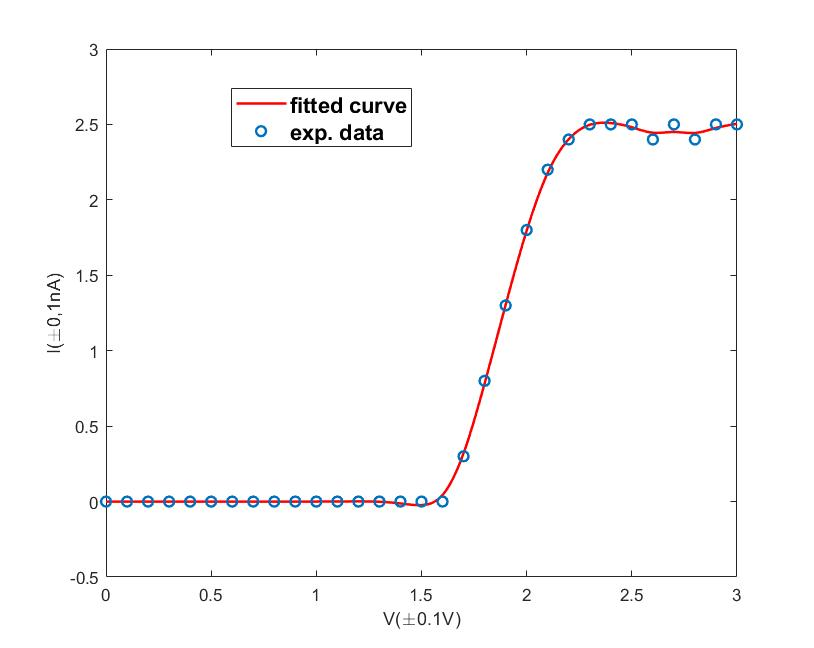
\includegraphics[width=0.9\linewidth]{plot1.jpg}
	 		\caption{ }
	 		\label{im1}
	 	\end{figure}
	 	
	 	Παρατηρώ ότι η τάση στην οποία αρχίζει η αύξηση του ρεύματος είναι περίπου $U_c = (1.6\pm0.1)V$ και παρ' όλου που είναι κοντά στην θεωρητική (1.8V) δεν την περιλαμβάνει στα όρια του σφάλματος.
	 	
	 	Αν τα ηλεκτρόνια διαφεύγουν από το πηγάδι δυναμικού που δημιουργούν τα δύο μέταλλα σε τάση $U_c$ και επιταχύνονται σε τάση $U_2 = U_1=(2.0\pm0.1)V$, τότε απομένει να επιταχυνθούν στα 0.4V, άρα $E_0 = (0.4\pm0.1)eV$
	 	
	 	
	\subsubsection*{Μέρος Β': Καμπύλη $I_3-U_2$}
			Τώρα θέτουμε την $U_1 = 2.0 V$ και την επιβραδυντική τάση $U_3 = -8.0V$. Αφού παρατηρήσουμε τις φωτεινές περιοχές, μετααβάλλουμε την $U_2$ από $0-80V$ και καταγράφουμε το ρεύμα στον δίσκο Δ3 για κάθε τιμή της τάσης. Το βήμα μεταβολής της $U_2$ είναι  1V γενικά και 0.5V στις περιοχές που περιμένουμε απότομη πτώση του ρεύματος στον Δ3.
			
			Τα αποτελέσματα φαίνονται στον Πίνακα (\ref{mat2}).
			
			\begin{table}[h!]
				\centering
				\begin{tabular}{r|r|||r|r|||r|r|||r|r}
				$U_2(\pm0.1V)$ & $I_3(\pm0.1nA)$ & $U_2(\pm0.1V)$ & $I_3(\pm0.1nA)$ & $U_2(\pm0.1V)$ & $I_3(\pm0.1nA)$ & $U_2(\pm0.1V)$ & $I_3(\pm0.1nA)$ \\\hline\hline
0.0&0.0&20.0&0.0&40.0&1.0&60.0&-0.5\\
1.0&0.1&20.5&0.2&41.0&1.3&61.0&-1.2\\
2.0&0.0&21.0&0.5&42.0&0.7&62.0&-2.1\\
3.0&0.0&22.0&0.7&43.0&-0.1&63.0&-3.2\\
4.0&0.0&23.0&0.8&44.0&-1.0&64.0&-4.5\\
5.0&0.1&24.0&0.7&45.0&-2.0&65.0&-5.9\\
6.0&0.1&25.0&0.1&46.0&-3.5&66.0&-7.4\\
7.0&0.1&26.0&-1.0&47.0&-3.7&67.0&-9.1\\
8.0&-0.2&27.0&-2.0&48.0&-4.5&68.0&-10.8\\
9.0&-0.9&28.0&-2.6&49.0&-5.1&69.0&-12.5\\
10.0&-1.4&29.0&-3.1&50.0&-5.7&70.0&-13.6\\
11.0&-1.7&30.0&-3.5&51.0&-6.3&71.0&-14.2\\
12.0&-1.9&31.0&-3.8&52.0&-6.3&72.0&-14.5\\
13.0&-2.1&32.0&-4.0&53.0&-5.5&73.0&-14.4\\
14.0&-2.2&33.0&-4.2&53.5&-5.1&74.0&-14.3\\
15.0&-2.4&34.0&-4.3&54.0&-4.6&74.5&-14.1\\
16.0&-2.5&34.5&-4.3&54.5&-3.9&75.0&-14.0\\
16.5&-2.6&35.0&-3.8&55.0&-3.4&75.5&-14.3\\
17.0&-2.7&35.5&-3.1&55.5&-2.9&76.0&-14.5\\
17.5&-2.7&36.0&-2.4&56.0&-2.4&77.0&-15.0\\
18.0&-2.3&36.5&-1.8&57.0&-1.4&78.0&-16.4\\
18.5&-1.7&37.0&-1.1&58.0&-0.5&79.0&-18.1\\
19.0&-1.0&38.0&-0.1&59.0&-0.5&80.0&-20.8\\
19.5&-0.5&39.0&0.5&0.0&0.0&0.0&0.0\\
				\end{tabular}
				\caption{ }
				\label{mat2}
			\end{table}
	
	Η γραφική παράσταση $I_3 - U_2$ φαίνεται στην Εικόνα (\ref{im2}): 
	
	\begin{figure}[h!]
		\centering
		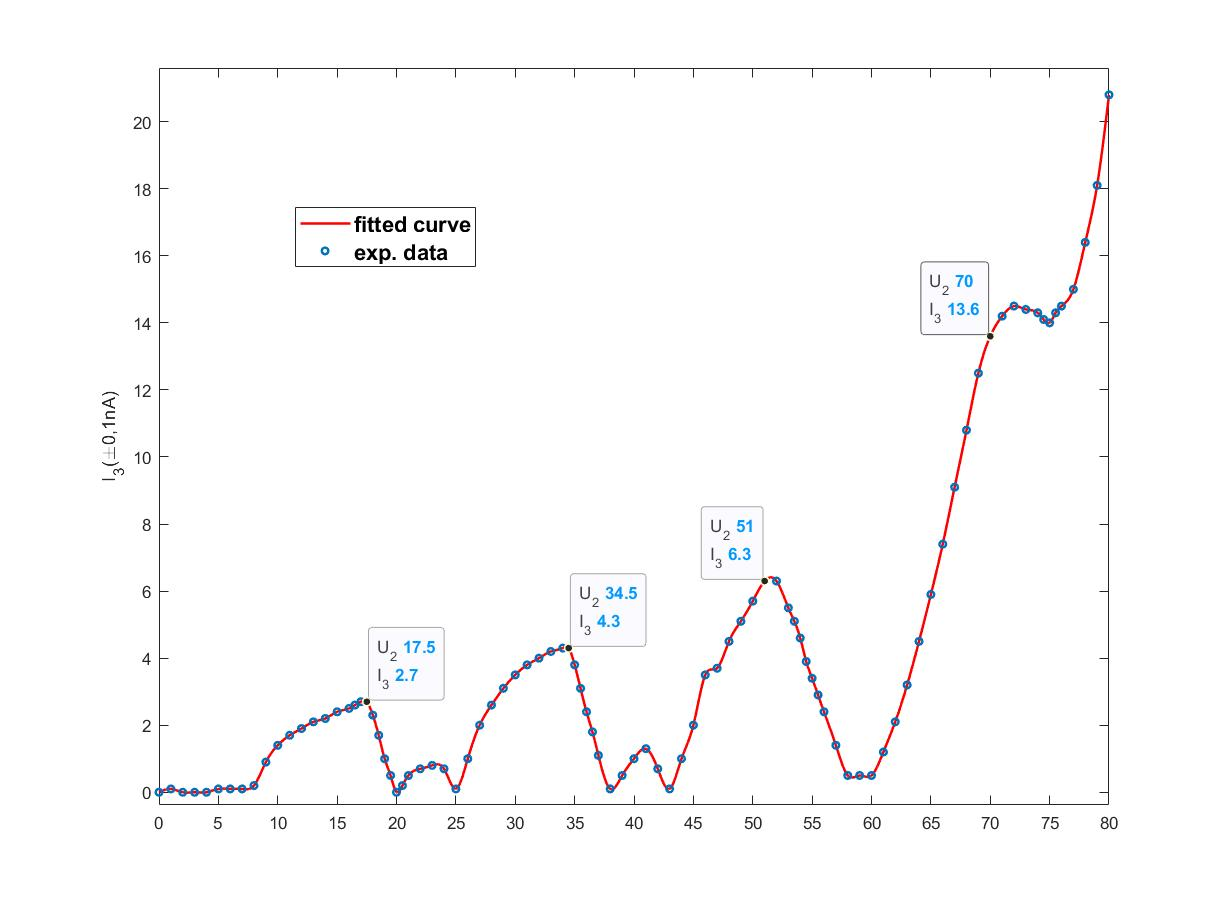
\includegraphics[width=1.2\linewidth]{plot2.jpg}
		\caption{ }
		\label{im2}
	\end{figure}
	
	Από την γραφική παράσταση παρατηρούμε πως η ανίχνευση μη μηδενικού ρεύματος $I_3$ ξεκινάει μετα τα 8V της τάσης καθώς για μικρότερες τιμές τα ηλεκτρόνια δεν μπορούν να ξεπεράσουν την επιβραδυντική τάση των $8V$. Στην περιοχή 8-17.5V το ρεύμα αυξάνεται καθώς στην κύρια περιοχή της λυχνίας έχουμε ελαστικές συγκρούσεις Νέου-ηλεκτρονίων. Όταν η τάση φτάσει μία κρίσιμη τιμή, τότε έχουμε πτώση του ρεύματος. Σε αυτή τη τιμή της τάσης τα ηλεκτρόνια έχουν τόση ενέργεια όση απαιτείται για να διεγείρουν το ηλεκτρόνιο του Νέου, θεωρτηικά αναμέναμε 16.7eV ενώ πειραματικά για την πρώτη διέγερση παρατηρούμε $(E_1)_1 = (17.5\pm0.1)eV$.
	
	Μετά από την παραπάνω τιμή της τάσης θα έπρεπε να παρατηρούμε μηδενισμό του ρεύματος καθώς τα ηλεκτρόνια έχοντας χάσει όλη τους την ενέργεια στην ανελαστική κρούση δεν μπορούν να ξεπεράσουν το επιβραδυντικό δυναμικό. Παρ' όλα αυτά παρατηρούμε ένα μικρότερο βουναλάκι ρεύματος. Αυτό οφείλεται στο γεγονός ότι το πεδίο στην επιφάνεια του Δίσκου Δ2 είναι ανομοιογενές και αυξάνεται όσο πλησιάζουμε τα άκρα των οπών. Δηλαδή, όσα ηλεκτρόνια περνούν κοντά από την περιφέρεια της κάθε οπής αποκτούν μεγαλύτερη κινητική ενέργεια από αυτά που περνούν από το κέντρο. Άρα όσα ηλεκτρόνια περνάνε μακριά από την περιφέρεια ενδέχεται να μην αποκτούν την απαιτούμενη ενέργεια για την διέγερση του Νέου άρα περνούν ανεμπόδιστα στην τρίτη περιοχή και τα ανιχνεύουμε ως $I_3$. Στην περιοχή της μείωσης του $I_3$ στην μιρκότερη κορυφή, το πεδίο στο εσωτερικό των οπών θα έχει αυξηθεί τόσο, ώστε όλο και περσσότερα ηλεκτρρόνια που περνούν όλο και πιό κοντά απ' το κέντρο θα είναι σε θέση να διεγείρουν το Νέο.
	
	Από το εύρος των μικρών κορυφών, μπορούμε να υπολογίσουμε την διαφορά δυναμικού κέντρου-περιφέρειας οπών. Από το πρώτο μικρό βουναλάκι παίρνουμε ένα εύρος $V_{κέντρο-περιφ,} = (5\pm0.5)V$.
	
	Έπειτα, για κάθε επόμενη μεγάλη κορυφή επαναλαμβάνονται τα ίδια φαινόμενα, απλώς καθώς αυξάνει η $U_2$ ''κάθε'' ηλεκτρόνιο προλαβαίνει να αποκτήσει δεύτερη, τρίτη φορά την απαιτούμενη ενέργεια για την διέγερση.
	
	Η ενέργεια διέγερσης $Ε_1$ είναι:%αν πάρουμε μέση τιμή των ενεργειών που είναι σημειωμένες διαιρεμένες με τον αριθμό της κορυφής που αντιστοιχεί (π.χ. θεωρητικά η δεύτερη κορυφή αντιστοιχεί σε $2E_1$, η τρίτη σε $3E_1$ κλπ) παίρνουμε: 
	\begin{align*}
		E_1 = ( 17.3 \pm 0.4 ) eV\footnotemark
	\end{align*}
\footnotetext{Χρησιμοποιώ το σφάλμα της γραφική που είναι $\delta V_i = 0.7\%V_i + 3\cdot0.1 $}
	
	Η πειραματική επιβεβαίωση του ότι τα ηλεκτρόνια έχουν μηδενική ενέργεια έπειτα από τις μη ελαστικές συγκρούσεις έγκειται στο ότι έπειτα από την απότομη πτώση του $I_3$, ξαναεμφανίζεται περίπου μετά από αύξηση της $U_2$ κατά 8V. Συνεπώς αν είχαν μη μηδενική κινητική ενέργεια θα ανιχνεύαμε ρεύμα $I_3$ για αύξηση της $U_2$ μικρότερω των 8V. 
	
	Πέραν της εμφάνισης των ενδιάμεσων μικρών κορυφών ρεύματος, μία άλλη διαφορά πειραματικής και θεωρητικής καμπύλης είναι τα ύψη των κορυφών ρεύματος που αξάνονται καθώς μεγαλώνει η τάση. Εξ' αρχής έχουμε αμελήσει τα ηλεκτρόνια με ενέργειες ίσες με την ενέργεια διέγερσης, που για στατιστικούς λόγους δεν συγκρούονται με τα άτομα Νέου. Αυτά, ενδέχεται να συγκρουστούν με τα άτομα Νέου όταν αποκτήσουν ακόμη μεγαλύτερη ενέργεια και όταν ξεπεράσουν την τιμή των 21.6eV τα ιονίζουν. Τότε εμφανίζοντια νέα ηλεκτρόνια στον κύριο χώρο τα οποία επιταχύνονται απ' το δυναμικό $U_2$ και γι' αυτό αυξάνεται το μέγιστο της κάθε κορυφής.
	
	\subsubsection*{Νανοαμπερόμετρο}
	
	Το κοινό αμπερόμετρο μετρά ρεύματα με ακρίβεια στο δέκατο του μικρομέτρου την στιγμή που εμείς θέλουμε δύο τάξεις μικρότερη. Γι' αυτό, τοποθετούμε μία αντίσταση 1ΜΩ στα άκρα του πολυμέτρου το οποίο θα χρησιμοποιήσουμε ως βολτόμετρο. Δεδομένου ότι η αντίσταση του βολτομέτρου είναι 100ΜΩ, θα περνάει από αυτή μονο το 1\% του ολικού ρεύματος και η πτώση τάσης θα είναι αντίστοιχα το 1\% αυτής που θα προκαλλούσε το συνολικό ρεύμα. Έτσι, αν η ακρίβεια του βολτομέτρου είναι 0.01μV, τότε από τον ν.Ohm $I=U/R =0.01nA$. 
	
	Επιπλεόν, συνδέουμε έναν πυκνωτή παράλληλα με την μετρητική αντίσταση 1ΜΩ, με στόχο να μειωθεί η επαγόμενη τάση απ' το εναλασσόμενο ρεύμα του δικτύου.
\end{document}